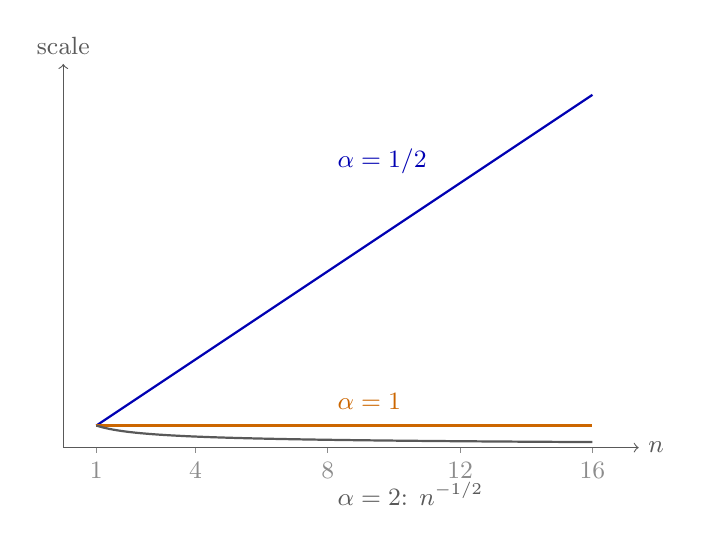
\begin{tikzpicture}[x=0.42cm,y=0.28cm]
\draw[->,black!65] (0,0)--(17.4,0) node[right,font=\small] {$n$};
\draw[->,black!65] (0,0)--(0,17.4) node[above,font=\small] {scale};
\draw[blue!70!black,thick] (1,1)--(16,16);
\draw[orange!80!black,thick] (1,1)--(16,1);
\draw[black!65,thick] plot[domain=1:16,samples=80] (\x,{1/sqrt(\x)});
\foreach \x in {1,4,8,12,16}{\draw[black!45] (\x,0)--(\x,-0.24) node[below,font=\small] {$\x$};}
\node[blue!70!black,font=\small,anchor=west] at (8,13) {$\alpha=1/2$};
\node[orange!80!black,font=\small,anchor=west] at (8,2.1) {$\alpha=1$};
\node[black!65,font=\small,anchor=west] at (8,-2.1) {$\alpha=2$: $n^{-1/2}$};
\end{tikzpicture}
